\documentclass{beamer}
\usepackage[latin1]{inputenc}
\usepackage{adjustbox}
\usetheme{Montpellier}
\usecolortheme{dove}

\title[Parameterization and Uncertainty in MD Simulations]
      {Exploring Parameterization and Uncertainty \\
       in Molecular Dynamics Simulations}
\author{Sean Laguna}
\institute{University of Chicago}
\date{Nov 13, 2013}
\begin{document}

\begin{frame}
\titlepage
\end{frame}

%%%

\begin{frame}{Describing the model}
What are the components of a Molecular simulation?
\end{frame}

\begin{frame}{Short, sweet answer}
\begin{itemize}
    \item A differential equation that models the system
    \item A set of constraints
    \item A set of initial conditions 
    \item A set of (somewhat) independent parameters
\end{itemize}
\end{frame}

%%%

\begin{frame}{The devil's in the details}
What does the DE represent and how is it formed?
\begin{itemize}
    \item A differential equation that models the system
\end{itemize}
\begin{center}
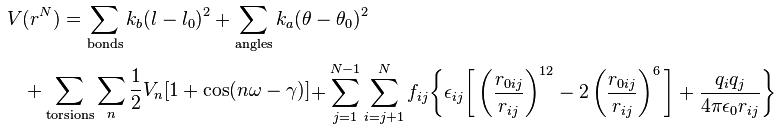
\includegraphics[width=0.78\textwidth]{images/AMBER}
\end{center}
\begin{itemize}
    \item This is actually a potential function...the force is the negative
        spatial derivative of this equation
    \item It ``doesn't matter'' what these parameters represent...the thing to
        notice is that there are a lot of them
\end{itemize}
{\footnotesize Cornell et. al, 1995}
\end{frame}

%%%

\begin{frame}{The devil's in the details}
What does the DE represent and how is it formed?
\begin{itemize}
    \item By studying the behavior of physical systems and...
    \begin{itemize}
        \item ...deriving a simple functional model for those behaviors
        \begin{itemize}
            \item (bond forces, angles, torsions, and unbonded forces)
        \end{itemize}
        \item ...fitting the parameters to experimental data or ab-initio
            calculations
        \begin{itemize}
            \item inform fast, large models with information from slow, small
                models (ideally, the small models will be accurate in general)
            \item huge level of parametric variation depending on the
                system; different parameter sets for nucleic acids/proteins
                (peptides), carbohydrates, etc
        \end{itemize}
    \end{itemize}
\end{itemize}
\end{frame}

%%%

\begin{frame}{Scale of functional units}
Constraints are described at various scales:
\begin{itemize}
    \item Whole molecules
    \item \textcolor{red}{Residues}
    \item Atoms/ions
    \item Subatomic (quantum-mechanical?)
Some scales are abstracted and integrated into others. For example, ions are
ultimately at the atomic scale but contain hard-coded information about their
subatomic composition.

\end{itemize}
\end{frame}

%%%

\begin{frame}{Residues}
Residue: "A residue is a building block for a larger polymeric material"
\begin{itemize}
    \item Residues are just sets of parameters and constraints for groups of atoms
    \item Water is a residue
    \item The hope is that these units are more or less general, and static
        throughout the course of the simulation
    \item Determining force field parameters for residues is an active research topic

\end{itemize}
\end{frame}

%%%

\begin{frame}
\begin{center}
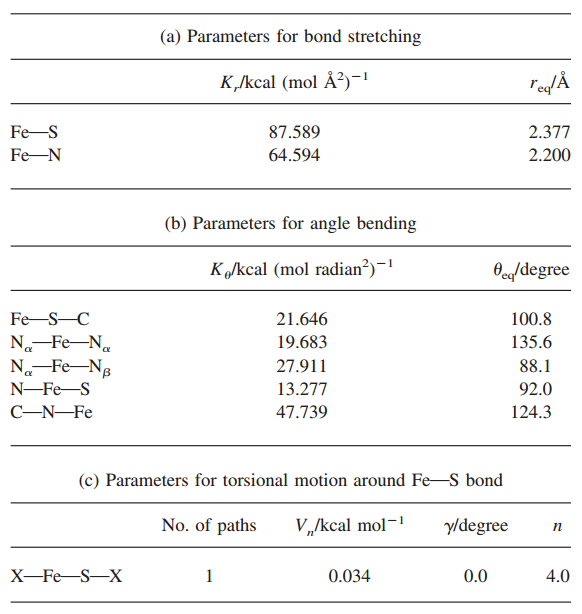
\includegraphics[width=0.4\textwidth]{images/iron_params} \\
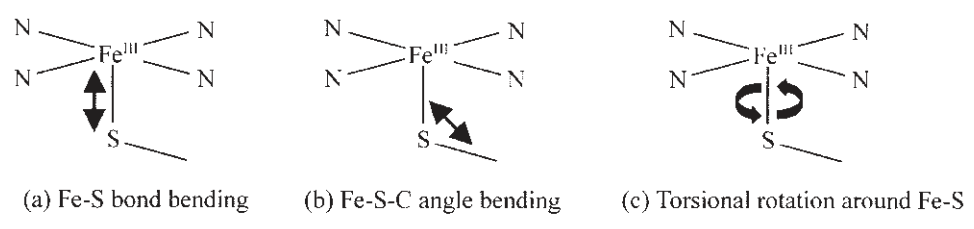
\includegraphics[width=0.8\textwidth]{images/iron_diags}
\end{center}
{\footnotesize Oda et. al, 2005}
\end{frame}

%%%

\begin{frame}[fragile]
\begin{tabular}{cc}
\begin{minipage}{0.5\textwidth}
{\scriptsize
\begin{verbatim}
[ NH2 ]
 [ atoms ]
     N    N   -0.46300    1
    H1    H    0.23150    2
    H2    H    0.23150    3
 [ bonds ]
     N   H1
     N   H2
    -C    N 
 [ impropers ]
    -C   H1    N   H2
\end{verbatim}
}
{\footnotesize AMBER03 rtp}
\end{minipage}
&
\begin{minipage}{0.5\textwidth}
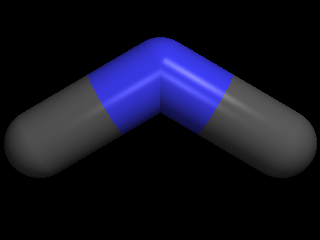
\includegraphics[width=0.8\textwidth]{images/amidogen}
\end{minipage}
\end{tabular}
\end{frame}

%%%

\begin{frame}[fragile]
\begin{tabular}{cc}
\begin{minipage}{0.5\textwidth}
{\scriptsize
\begin{verbatim}
; tip3p
[ HOH ]
 [ atoms ]
    OW   OW   -0.834    0
   HW1   HW    0.417    0
   HW2   HW    0.417    0
 [ bonds ]
    OW   HW1
    OW   HW2
\end{verbatim}
}
{\footnotesize AMBER03 rtp}
\end{minipage}
&
\begin{minipage}{0.5\textwidth}
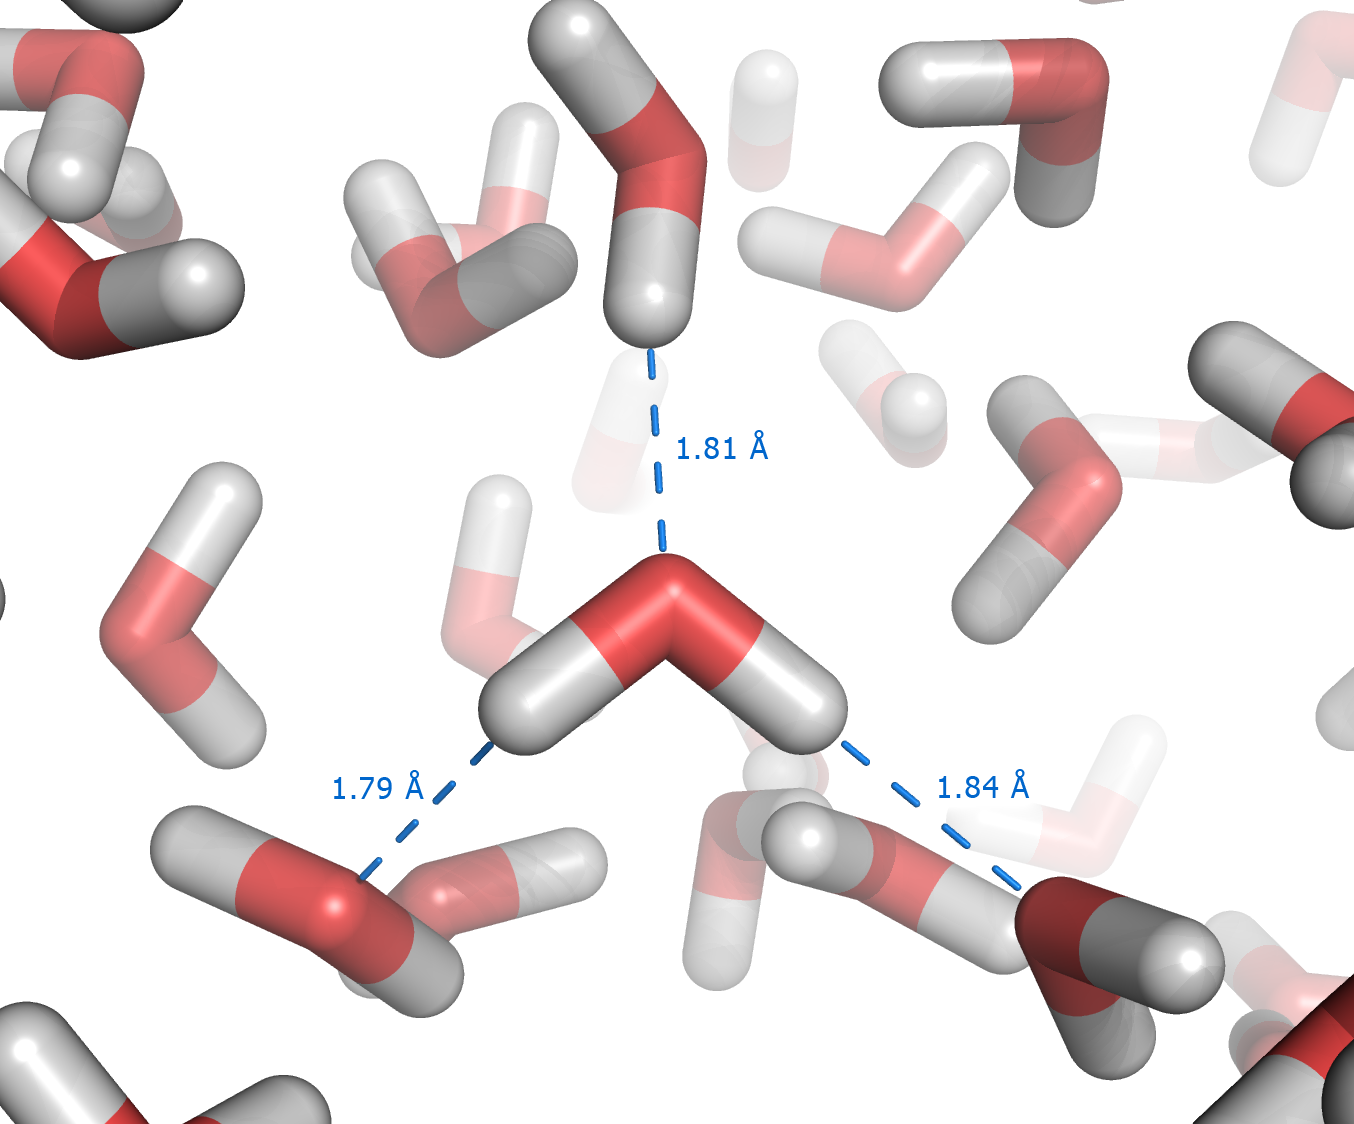
\includegraphics[width=0.8\textwidth]{images/tip3p}
\end{minipage}
\end{tabular}
\end{frame}

%%%

\begin{frame}{IC/BCs and (independent) parameters}
Residue: "A residue is a building block for a larger polymeric material"
\begin{itemize}
    \item Initial configuration of system, timestep, cutoff radii, etc
    \item How do they interact with the rest of the model?
    \begin{itemize}
        \item Requires domain-specific knowledge and experimentation to know
    \end{itemize}
    \item Also, a variety of methods exist for NPT/NVT etc simulations, energy
        minimization
    \item Some water models have been built for specific
        methods/quantities of interest, e.g. Ewald summation for computing
        interaction energies of periodic systems (Price et. al, 2004)
\end{itemize}
\end{frame}

%%%

\begin{frame}
Q: If I want to improve the accuracy of some quantity of my model, which
parameters do I adjust?
\end{frame}

%%%

\begin{frame}
A1: All of them. Build a heuristic model specifically for your system. Specify
all of the residues and their parameters, tweak existing residues and parameters
to match experimental data for your particular system, and change parameters if
your results don't match experimental data.
\end{frame}

%%%

\begin{frame}
    \Huge{Overfitting}
\end{frame}

%%%

\begin{frame}
A2: Determine what portion of your model is contributing to the error. Compute
or find (in a paper somewhere) improved ab-initio calculations for certain
residues, and implement them alongside a generic force fifeld and at the
smallest possible scale. Implement them modularly alongside the use of a generic
force field. Use flexible models instead of rigid ones. Do error analysis on
your system to determine an appropriate time step and appropriate cutoff radii.
Generic models should work, already-verified theories should work, statistical
analysis is a legitimate thing, etc!
\end{frame}

%%%

\begin{frame}
When people do this, it doesn't always work...\\[\baselineskip]
Even the best models are inaccurate for very small systems...\\[\baselineskip]
Dynamic computation is much slower than static data...\\[\baselineskip]
Not to mention that doing this well is extremely challenging...\\[\baselineskip]
\end{frame}

%%%

\begin{frame}{Comparing SPC/E to TIP3P}
    \begin{center}
    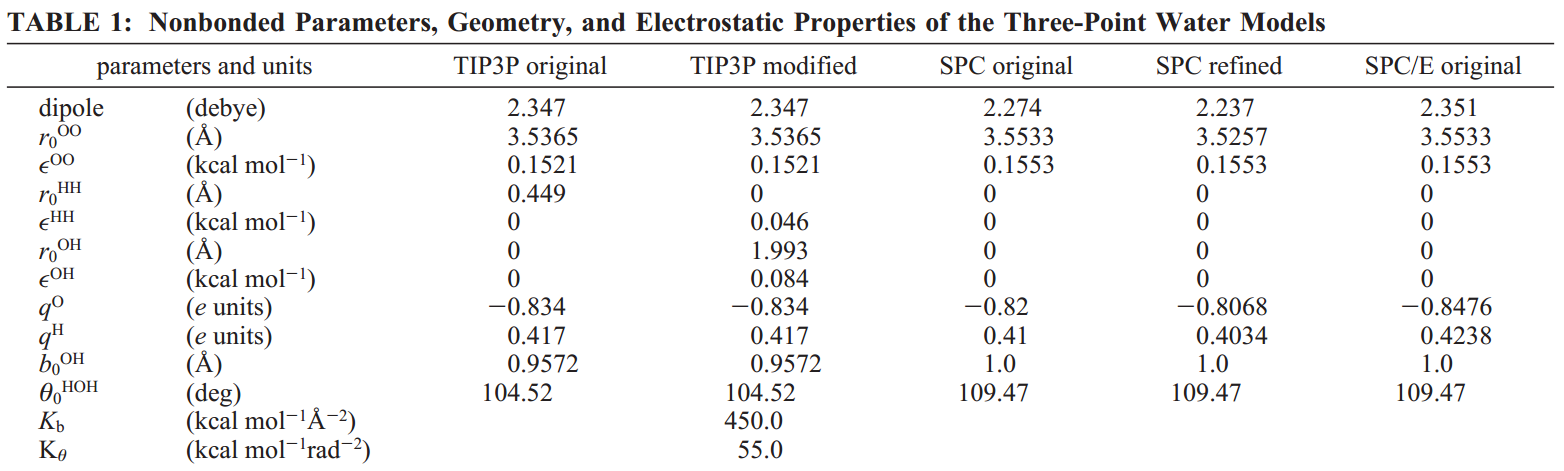
\includegraphics[width=0.98\textwidth]{images/watercomp_params.png}
    \end{center}
{\footnotesize Mark and Nilsson, 2001}
\end{frame}
\begin{frame}{Comparing SPC/E to TIP3P}
    \begin{center}
    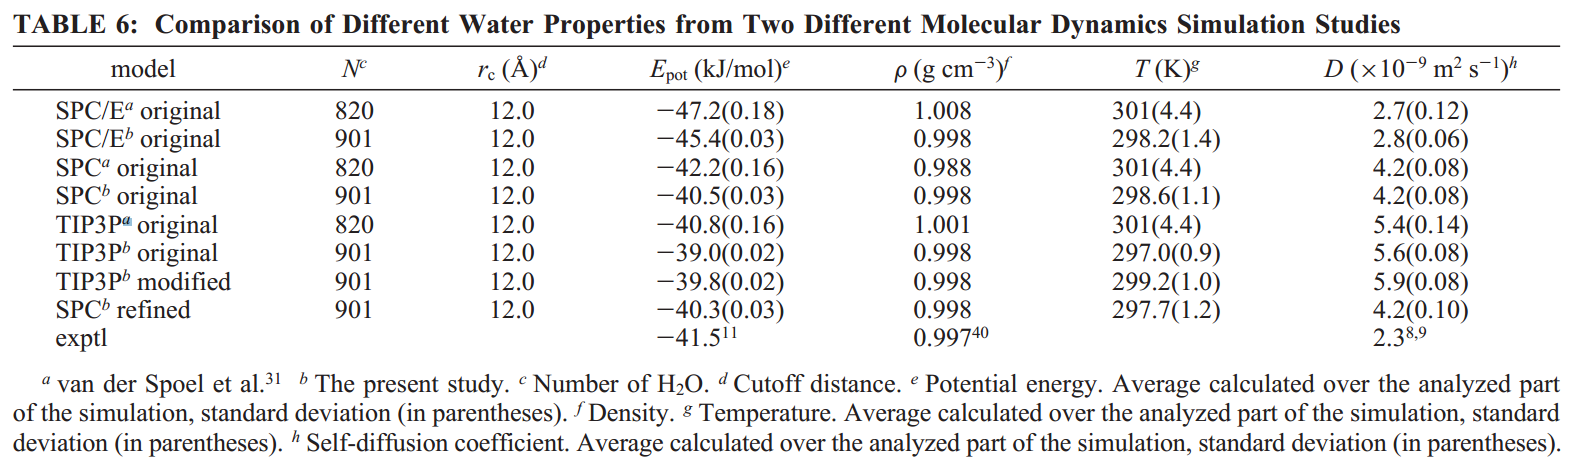
\includegraphics[width=0.98\textwidth]{images/watercomp_props.png}
    \end{center}
{\footnotesize Mark and Nilsson, 2001}
\end{frame}
\begin{frame}{Comparing SPC/E to TIP3P}
    \begin{center}
    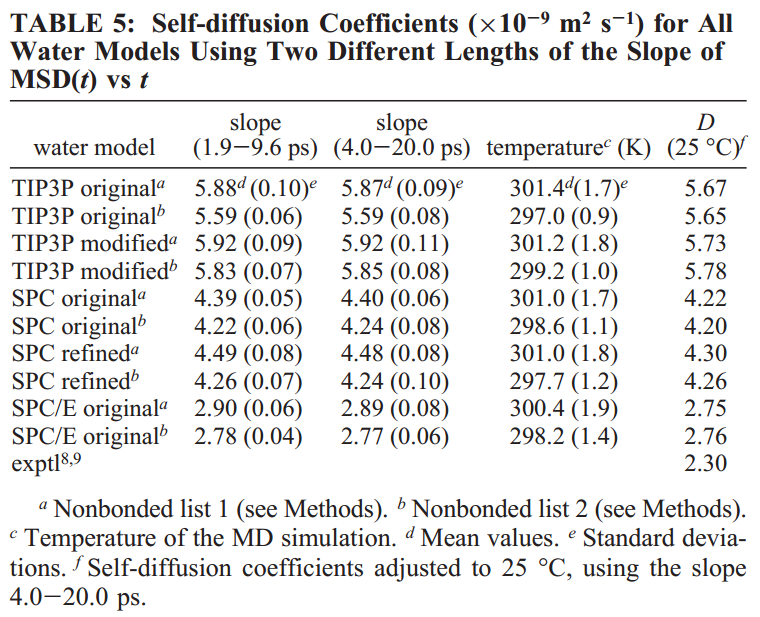
\includegraphics[width=0.55\textwidth]{images/watercomp_selfdiff.png}
    \end{center}
{\footnotesize Mark and Nilsson, 2001}
\end{frame}
\begin{frame}{Comparing SPC/E to TIP3P}
    \begin{center}
    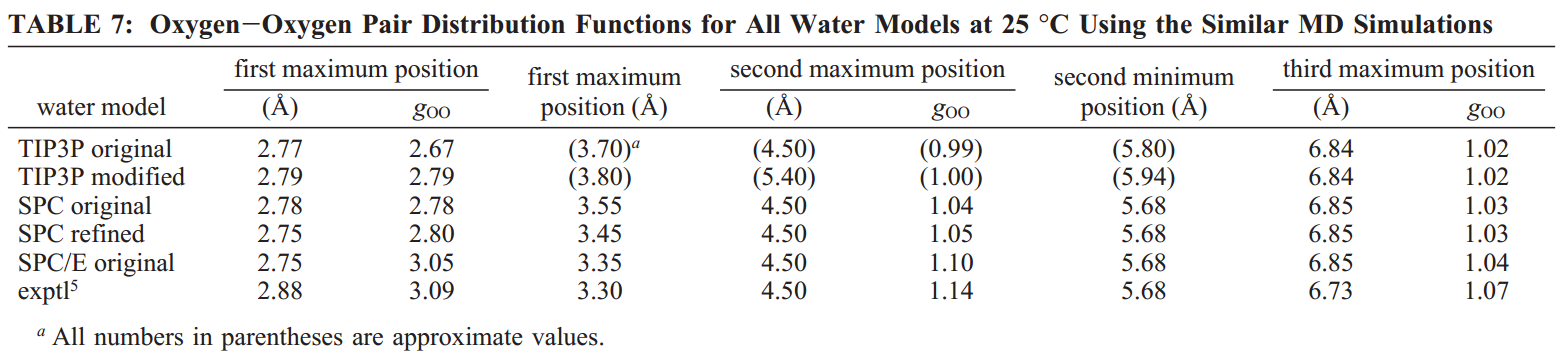
\includegraphics[width=0.98\textwidth]{images/watercomp_rdfsOO.png} \\
    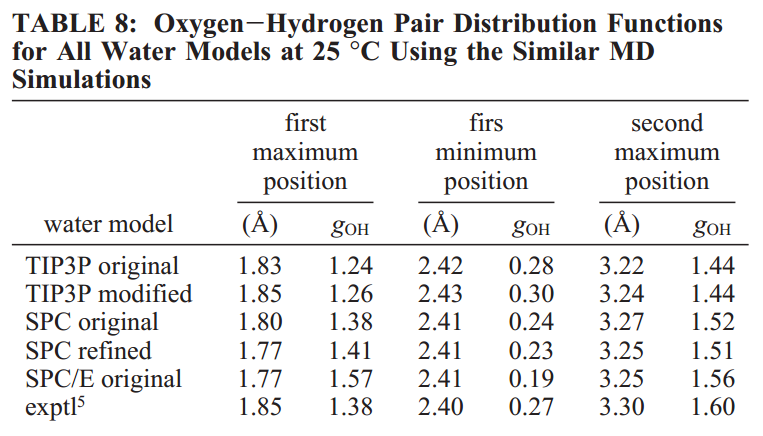
\includegraphics[width=0.55\textwidth]{images/watercomp_rdfsOH.png}
    \end{center}
{\footnotesize Mark and Nilsson, 2001}
\end{frame}

\begin{frame}{Takeaway}
Amending the force field significantly improves the correspondence between the
model and experimental data. \\[\baselineskip]
But, it forces some unphysical parameters.
\end{frame}

\begin{frame}{Takeaway}
\Huge{Atoms don't have point charges! They have probability distributions of
electrons.}
\end{frame}

\begin{frame}{Solutions? GCPM}
Treat atom/site charge as a distribution
    \begin{itemize}
        \item Gaussian Charge Polarizable Model
        \item Mathematically reasonable...programmatically ugly
        \item Recovers some properties very nicely, others, not so much
    \end{itemize}
    \begin{tabular}{cc}
    \begin{minipage}{0.38\textwidth}
    \begin{center}
        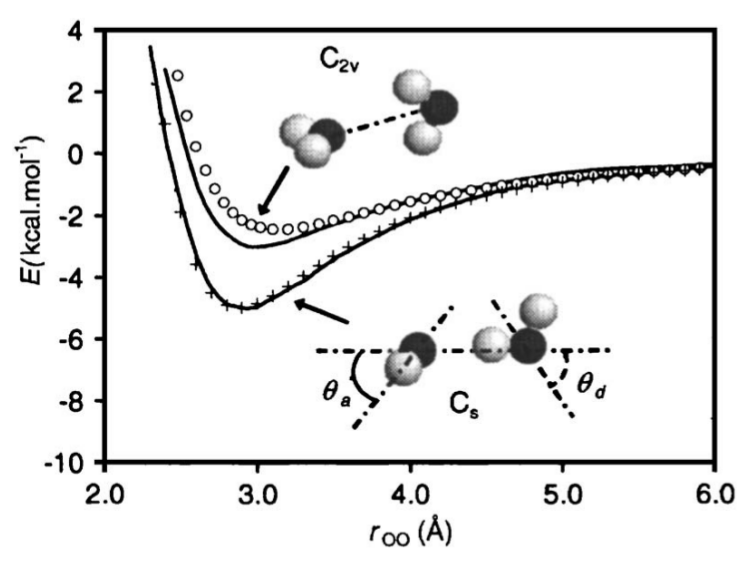
\includegraphics[width=0.98\textwidth]{images/gcpm_dimer.png} \\
    \end{center}
    \end{minipage}
    &
    \begin{minipage}{0.62\textwidth}
        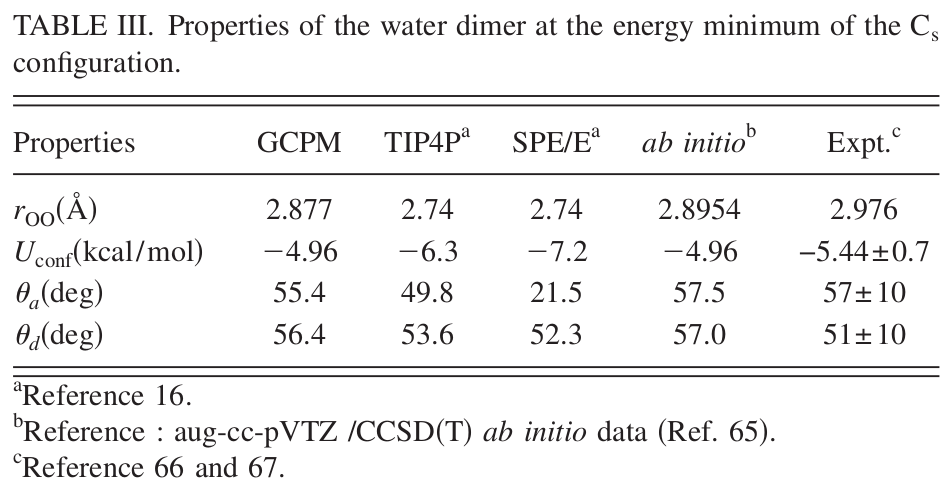
\includegraphics[width=0.92\textwidth]{images/gcpm_compFull.png} \\
    \end{minipage}
    \end{tabular}
    {\footnotesize Paricaud et. al, 2005}
\end{frame}

\begin{frame}
    \begin{center}
    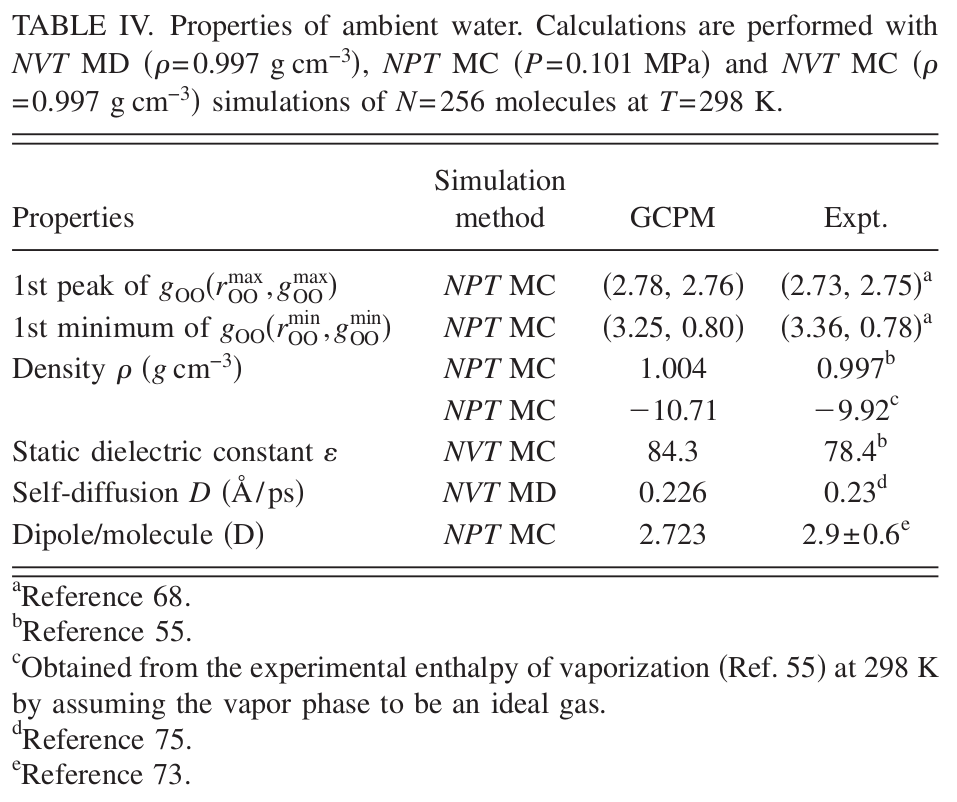
\includegraphics[width=0.78\textwidth]{images/gcpm_compExp.png}
    \end{center}
\end{frame}

\begin{frame}{Solutions?}
Use a continuum model
    \begin{itemize}
        \item Relate (coarse-grain) the microscopic charge density to
            the macroscopic charge density
        \item Calculate the polarization field and resulting force
            field, and include it in the overall force field for the
            model
        \item Good for recovering bulk properties of water and tuning
            accuracy, bad for looking at properties of individual
            molecules
            \begin{itemize}
                \item (At the very least...it has not been yet used for
                    this purpose...)
                \item \textbf{Computed bulk dielectric constant of water} \\
                    \scriptsize{GCPM: $84 \pm 15$ \\
                        Continuum: $72 \pm3$ [1] \\ 
                        TIP3P: $84-112$ (for various parameter tunings) [2] \\
                    experimental: $78.9$ [3]}
            \end{itemize}
    \end{itemize}
    \footnotesize{ 
        {[}1{]} Mandapu, Templeton, and Lee, 2013 \\
        {[}2{]} Price and Brooks, 2004 \\
        {[}3{]} Abeyrathne et. al, 2013 \\}
\end{frame}


%%%

%\begin{frame}{Conclusion}


\end{document}
